\documentclass[12]{article}
\usepackage{graphicx}
\usepackage{color}
\usepackage{algorithmic}
\begin{document}

\title{\textbf{\\
\textcolor{red}{Universitatea din Craiova \\Facultatea de Automatic\u{a},Calculatoare \c{s}i Electronic\u{a}}}}
\date{\textbf{5.iunie.2018}}
\maketitle
\begin{center}
\end{center}
\textbf{Proiect : Inteligenta Artificiala} \\
\textbf{Titlu : Tic Tac Toe }\\
\textbf{Student : Voica Catalin Gabriel} \\
\textbf{Sectie : Calculatoare Romana\u{a}\\ Anul 2\\ Grupa : CR 2.1 C}
\newpage
\tableofcontents

\newpage
\section{Declararea Problemei}

\textcolor{white}{}
\subsection{Titlu}
Tic Tac Toe

\subsection{Descriptie}
\textcolor{white}{}


Pentru proiectul meu a trebuit sa implementez jocul Tic Tac Toe (X si  0),iar apoi sa testez si sa  evaluez performanta a doua algoritme de cautare euristice.Cele doua functii euristice pe care trebuia sa le fac sunt A* Search si Recursive Best First Search.
\newline
\newline

La algoritmul pe care trebuie sa il implementez se vor verifica urmatoarele lucruri:
-Verificarea completitudinii : daca algoritmul respectiv determina o solutie,cate solutii poate gasi algoritmul.
-Verificarea optimitatii:se va verifica daca algoritmul determina o solutie optima cand exista cel putin o solutie.Se va verifica deasemenea si daca algoritmul respectiv determina solutia optima din prima incercare.
-Complexitatea Timpului:cat timp dureaza sa gaseasca o solutie si/sau solutia optima.
\newline
\newline

Se cere sa se implementeze seturi de date nontriviale care sa contina cel putin 10 cazuri de teste de marimi variabile :mici,medii,mari si foarte mari astfel incat fisierele de date sa incapa intr-o arhiva de 8 MB.Fiecare caz de test trebuie sa defineasca starea spatiului,dar si valoarea functiei euristice pentru fiecare stare.
\newline
\newline 

La aplicatia pe care trebuia sa o implementez,Tic Tac Toe,nu am reusit sa aplic niciuna dintre cele doua functii euristice,A* Search si Recursive Best First Search.In shimb am reusit sa termin jocul,construind o clasa "checkRules" care contine cate o functie pentru fiecare caz in care jocul Tic Tac Toe se poate termina,o clasa "board"  prin care se introduc mutarile jucatorului,mutarile acestuia fiind simulate de catre program.Tot in clasa "board" se actualizeaza jocul la fiecare mutare a jucatorului,urmand apoi sa se faca afisarea.La final am mai construit o clasa "gameRules" care sa ruleze functiile care verifica daca jocul s-a terminat sau nu.La sfarsitul jocului simulat,aceasta clasa va afisa rezultatul final.

Proiectul s-a ales in functie de formula 1 + (suma codului ASCII al numelui de familie + primul prenume modulo 5)

voica catalin (v - 118,o-111,i-105,c-99,a-97,space-32,c-99,a-97,t-116,a-97,l-108,i-105,n-110)

Formula : ((118+111+105+99+97+32+99+97+116+97+108+105+110)mod5) + 1 = 5 (a rezultat problema 5)



\newpage
\section{Pseudocod}

\subsection{board checkWhoStarts()}
\begin{algorithmic}[1]
\STATE randomize v1

\IF {v1 == 1}
	\STATE return 1;
\ENDIF
	\STATE return 0;

\end{algorithmic}

\subsection{board playGame (n,matrix,currentPlayer,playerChoice)}
\begin{algorithmic}[1]
\STATE randomize line
\STATE randomize column

\WHILE { $matrix[line][column] \neq $0 or $ line \geq $n or$ column \geq $n or $line \geq $n and $column \geq $n}
	\IF{$line \geq $n or$ column \geq $n or $line \geq $n and $column \geq $n}
		\STATE randomize line
		\STATE randomize column
	\ENDIF
	
	\IF {$matrix[line][column] \neq $0}
		\STATE randomize line
		\STATE randomize column
	\ENDIF
\ENDWHILE

\IF {currentPlayer == 1 and playerChoice == 1}
	\STATE $matrix[line][column] \gets $playerChoice
	\STATE updateMatrix(n,matrix,playerChoice)
\ENDIF

\IF {currentPlayer == 2 and playerChoice == 2}
	\STATE  $matrix[line][column] \gets $playerChoice
	\STATE updateMatrix(n,matrix,playerChoice)
\ENDIF
 
\end{algorithmic}

\subsection{board updateMatrix (n,matrix,playerChoice)}
\begin{algorithmic}[1]
\FOR {$i = $0 \TO n}
	\FOR {$j = $0 \TO n}
		\IF{$matrix[i][j] \neq $ 1 and $matrix[i][j] \neq $2}
			\STATE $ matrix[i][j] \gets $0
		\ENDIF
			\STATE $matrix[line][column] \gets $playerChoice
	\ENDFOR
\ENDFOR

\end{algorithmic}

\subsection{board showMatrix (n,matrix)}
\begin{algorithmic}[1]

\FOR {$ i = $0 \TO n}
	\FOR {$j = $0 \TO n}
		\STATE print matrix[i][j]
	\ENDFOR
	
\ENDFOR

\end{algorithmic}

\subsection{checkRules checkIfBoardFull(n,matrix)}
\begin{algorithmic}[1]

\STATE $k \gets $0

\FOR {$ i = $0 \TO n}
	\FOR {$j = $0 \TO n}
		\IF{matrix[i][j] == 0}
			\STATE $k \gets $k + 1
		\ENDIF
	\ENDFOR
	\IF{k==0}
		\STATE return 0
	\ENDIF
		\STATE return 1
\ENDFOR
\end{algorithmic}




\subsection{checkRules checkTheLines(n,matrix,playerchoice)}
\begin{algorithmic}[1]

\IF{playerChoice == 1}
	\STATE $k \gets $0
	\FOR {$ i = $0 \TO n}
		\FOR {$j = $0 \TO n}
			\IF{$matrix[i][j] \neq $playerChoice and $k < $n and j == n-1}
				\STATE $k \gets $0
			\ENDIF
			\IF{matrix[i][j] == playerChoice and $k < $n}
				\STATE $k \gets $0 
				\IF{k==n}
					\STATE $save \gets $i
				\ENDIF
				\IF{j ==  n-1 and $k < $n}
					\STATE $k \gets $0
				\ENDIF
			\ENDIF
		\ENDFOR
	\ENDFOR
	\IF{k==n}
		\STATE return 1
	\ENDIF
		\STATE return 0
\ENDIF

\IF{playerChoice == 2}
	\STATE $k \gets $0
	\FOR {$ i = $0 \TO n}
		\FOR {$j = $0 \TO n}
			\IF{$matrix[i][j] \neq $playerChoice and $k < $n and j == n-1}
				\STATE $k \gets $0
			\ENDIF
			\IF{matrix[i][j] == playerChoice and $k < $n}
				\STATE $k \gets $0 
				\IF{k==n}
					\STATE $save \gets $i
				\ENDIF
				\IF{j ==  n-1 and $k < $n}
					\STATE $k \gets $0
				\ENDIF
			\ENDIF
		\ENDFOR
	\ENDFOR
	\IF{k==n}
		\STATE return 1
	\ENDIF
		\STATE return 0
\ENDIF

\end{algorithmic}

\subsection{checkRules checkTheColumns(n,matrix,playerChoice)}
\begin{algorithmic}[1]

\IF{playerChoice==1}
	\STATE $k \gets $0
	\FOR{$i = $0 \TO n}
		\FOR{$j = $0 \TO n}
			\IF{matrix[i][j] == playerChoice and $k < $n and i == 0 or ($matrix[i][j] \neq $playerChoice and $k < $n and i==0)}
				\STATE $k \gets $0
			\ENDIF
			\IF{matrix[i][j] == playerChoice and $k < $n}
				\STATE $k \gets $k+1
					\IF{k==n}
						\STATE $save \gets $j
					\ENDIF
			\ENDIF
		\ENDFOR
	\ENDFOR
	\IF{k==n}
		\STATE return 1
	\ENDIF
		\STATE return 0
\ENDIF

\IF{playerChoice==2}
	\STATE $k \gets $0
	\FOR{$i = $0 \TO n}
		\FOR{$j = $0 \TO n}
			\IF{matrix[i][j] == playerChoice and $k < $n and i == 0 or ($matrix[i][j] \neq $playerChoice and $k < $n and i==0)}
				\STATE $k \gets $0
			\ENDIF
			\IF{matrix[i][j] == playerChoice and $k < $n}
				\STATE $k \gets $k+1
					\IF{k==n}
						\STATE $save \gets $j
					\ENDIF
			\ENDIF
		\ENDFOR
	\ENDFOR
	\IF{k==n}
		\STATE return 1
	\ENDIF
		\STATE return 0
\ENDIF


\end{algorithmic}

\subsection{checkRules checkTheDiagonalOne(n,matrix,playerChoice)}
\begin{algorithmic}[1]

\IF {playerChoice == 1}
	\STATE $k \gets $0
	\FOR{$i = $0 \TO n}
		\FOR{$j=$0 \ TO m}
			\IF{i==j and matrix[i][j] == playerChoice}
				\STATE $k \gets $0
			\ENDIF
		\ENDFOR
	\ENDFOR
\ENDIF
\IF{k==n}
	\STATE return 1
\ENDIF
	\STATE return 0
\IF {playerChoice == 2}
	\STATE $k \gets $0
	\FOR{$i = $0 \TO n}
		\FOR{$j=$0 \ TO m}
			\IF{i==j and matrix[i][j] == playerChoice}
				\STATE $k \gets $0
			\ENDIF
		\ENDFOR
	\ENDFOR
\ENDIF
\IF{k==n}
	\STATE return 1
\ENDIF
	\STATE return 0


\end{algorithmic}

\subsection{checkRules checkTheDiagonalTwo(n,matrix,playerChoice)}
\begin{algorithmic}[1]

\IF{playerChoice == 1}
	\STATE $k \gets $0
	\STATE $i \gets $0
	\STATE $j \gets $n-1
	\WHILE{$i < $n and $j \geq $0}
		\IF{matrix[i][j] == playerChoice}
			\STATE $k \gets $k+1
		\ENDIF
		\STATE $i \gets $i+1
		\STATE $i \gets $j-1	
	\ENDWHILE
	\IF{k==n}
		\STATE return 1
	\ENDIF
		\STATE return 0
\ENDIF

\IF{playerChoice == 2}
	\STATE $k \gets $0
	\STATE $i \gets $0
	\STATE $j \gets $n-1
	\WHILE{$i < $n and $j \geq $0}
		\IF{matrix[i][j] == playerChoice}
			\STATE $k \gets $k+1
		\ENDIF
		\STATE $i \gets $i+1
		\STATE $i \gets $j-1	
	\ENDWHILE
	\IF{k==n}
		\STATE return 1
	\ENDIF
		\STATE return 0
\ENDIF

\end{algorithmic}

\subsection{gameRules checkTheGame(n,matrix,playerChoice,currentPlayer)}
\begin{algorithmic}[1]

\IF{checkTheLines(n,matrix,playerChoice) == 1}
	\STATE showMatrix(n,matrix)
	\STATE return 0
\ENDIF
\IF{checkTheColumns(n,matrix,playerChoice)==1}
	\STATE showMatrix(n,matrix)
	\STATE return 0
\ENDIF
\IF{checkTheDiagonalOne(n,matrix,playerChoice)==1}
	\STATE showMatrix(n,matrix)
	\STATE return 0
\ENDIF
\IF{checkTheDiagonalTwo(n,matrix,playerChoice)==1}
	\STATE showMatrix(n,matrix)
	\STATE return 0
\ENDIF
\IF{checkIfBoardFull(n,matrix)==0}
	\STATE showMatrix(n,matrix)
	\STATE return 0
\ENDIF

 
\STATE return 1

\end{algorithmic}

\newpage
\section{Designul Aplicatiei}
\subsection{Main}
\textbf{}
\newline

In functia main  primul lucru pe care l-am facut a fost sa initializez toate casutele din jocul Tic Tac Toe cu cifra '0',presupunand ca acele casute sunt casutele care nu sunt ocupate,jucatorii urmand sa le completeze ulterior(Jucatorul 1 joaca cu cifra '1' iar Jucatorul 2 joaca cu cifra '2').Tot in functia main se va stabili prin functia "checkWhoStarts" din clasa "board" care jucator va incepe primul,apoi va urma un while care va rula functia "checkTheGame" din interiorul clasei "gameRules" pana cand aceasta va returna 0,adica atunci cand una din conditiile ca jocul Tic Tac Toe sa se termine este indeplinita.

\subsection{Input Data}
\textcolor{white}{}

Ca input am ales functia "playGame" din clasa "board" sa dea valori aleatorii pentru numarul casutei care va fi selectata de unul din cei doi jucatori,aceasta generand numere aleatorii intre 0 si numarul de casute dorit pentru jocul de X si 0.Jocul de Tic Tac Toe pe care l-am dezvoltat poate rula pe n casute,numarul acestora stabilindu-se la inceputul functiei "main".

\subsection{Output Data}
\textcolor{white}{}

Atunci cand programul a terminat de rulat se va afisa pe ecran un joc de X si 0 pe n x n casute,casutele fiind completate de catre playeri,programul mentionand ce jucator a castigat,dar si pe ce linie,coloana sau diagonala a reusit acest lucru.Daca nici un jucator nu a castigat programul va mentiona acest lucru.

\subsection{Clasa board}

\subsubsection{checkWhoStarts}
\textcolor{white}{}

Functia "checkWhoStarts" din clasa "board" are rolul de a decide ce jucator va incepe primul jocul de X si 0,programul generand un numar la intamplare,acest numar poate sa fie '1' (caz in care incepe primul jucator) sau numarul '2' (caz in care va incepe al doilea jucator).

\subsubsection{playGame(n,matrix,currentPlayer,playerChoice}
\textcolor{white}{}

Functia "playGame" din clasa "board" are rolul de a completa casutele din interioriul matricei,in interioriul functiei generandu-se numere aleatorii.Functia deasemenea verifica daca vreo casuta din interioriul matricei a fost completata,sau daca numerele generate sunt prea mari decat capacitatea matricei respective,cazuri in care va genera alte numere.Tot din interioriul acestei functii se va actualiza si matricea dupa fiecare mutare a jucatorilor.

\subsubsection{updateMatrix(n,matrix,playerChoice)}
\textcolor{white}{}

Functia "updateMatrix" din clasa "board" are rolul de a actualiza matricea respectiva,dupa ce unul din jucatori a ales casuta din interioriul matricei.Aceasta functie este apelata din interiorul functiei "playGame" din aceeasi clasa.

\subsubsection{showMatrix(n,matrix)}
\textcolor{white}{}

Functia "showMatrix" din clasa "board" este apelata din clasa "gameRules".Functia este apelata in momentul in care una din conditiile pentru a se termina jocul a fost indeplinita,functia urmand sa afiseze rezultatul final al jocului de X si 0.

\subsection{Clasa checkRules}
\subsubsection{checkIfBoardFull(n,matrix)}
\textcolor{white}{}

Aceasta functie are rolul de a verifica daca  mai sunt mutari posibile,si niciun jucator nu a reusit sa invinga.In acest caz se,nu va mai exista nici o casuta goala (nu va mai exista cifra '0' in matrice la rezultatul final).Aceasta functie este apelata din interiorul functiei "checkTheGame" din clasa "gameRules.Aceasta functie este una din conditiile pe care eu le-am pus pentru a incheia jocul.(1/5)


\subsubsection{checkTheLines(n,matrix,playerChoice)}
\textcolor{white}{}

Aceasta functie este una din cele 5 functii pe care le-am folosit pentru a verifica daca jocul s-a terminat,functia avand rolul de a verifica pe linie daca mutarile jucatorului (cifra '1' sau '2') sunt egale cu n.Aceasta functie este si ea apelata tot din interiorul functiei "checkTheGame".(2/5)

\subsubsection{checkTheColumns(n,matrix,playerChoice)}
\textcolor{white}{}

Functia are acelasi rol ca functia precedenta,"checkTheLines",diferenta consta in faptul ca aceasta verifica daca unul din jucatori are numarul de mutari (cifra '1' sau '2') egal cu n.(3/5)

\subsubsection{checkTheDiagonalOne(n,matrix,playerChoice)}
\textcolor{white}{}

Cu aceasta functie se verifica pe prima diagonala (din coltul din stangas sus pana in coltul din dreapta jos) daca numarul de mutari al jucatorului (cifra '1' sau '2') este egala cu n.(4/5)

\subsubsection{checkTheDiagonalTwo(n,matrix,playerChoice)}
\textcolor{white}{}

Aceasta functie este ultima din cele 5 conditii ca jocul sa se incheie,si are rolul de a verifica pe a doua diagoanala (din coltul din dreapta de sus pana in coltul din stanga jos) daca numarul de mutari al jucatorului (cifra '1' sau '2') este egal cu n.(5/5)

\subsection{clasa checkRules}
\subsubsection{checkTheGame(n,matrix,playerChoice,currentPlayer)}
\textcolor{white}{}

Este functia care detine rolul cel mai important din program,aflandu-se in clasa "gameRules".Aceasta functie este apelata din interiorul functiei Main,este apelata in interiorul unui while,aceasta functie rulandu-se pana cand va returna 0.Se va returna valoarea 0 atunci cand una din cele 5 conditii pe care le-am prezentat mai sus va fi indeplinita.Tot din interiorul acestei functii se va apela si functia "showMatrix" in momentul in care jocul se va incheia.

\subsection{Concluzii}
\textcolor{white}{}

In concluzie mi s-a parut foarte interesant proiectul de facut la Inteligenta Artificiala,reusind sa imi fac o idee despre cum gandeste un calculator in momentul in care o persoana interactioneaza cu acesta,spre exemplu daca se joaca chiar X si 0.Prin cele doua euristici pe care ar fi trebuit sa le impllementez,programul este mai "destept",generand o serie de cautari,in care el incearca sa gaseasca solutia optima,devenind tot mai dificl pentru acea persoana sa ii faca fata.

\subsection{Referinte}
\textcolor{white}{}

\textbf{Book}:

$1.Stuart Russel - Artificial Intelligence: A Modern Approach$


\newpage
\section{Source Code}

\textcolor{white}{}

Proiectul meu s-a numit "n size Tic-Tac-Toe Game" .Am ales sa folosesc limbajul de programare C++,si am folos Visual Studio 2015.

\section{Experimente si rezultate}
\textcolor{white}{}

In prima poza,jucatorul 1(cel care joaca cu cifra '1') invinge,avand pe coloana a treia 3 de 1.
In cea de a doua poza,jucatorul 1 invinge,avand 1 pe diagonala.
In cea de a treia poza,cei doi jucatori termina la egalitate,nu mai exista casute goale (nu mai e cifra '0').


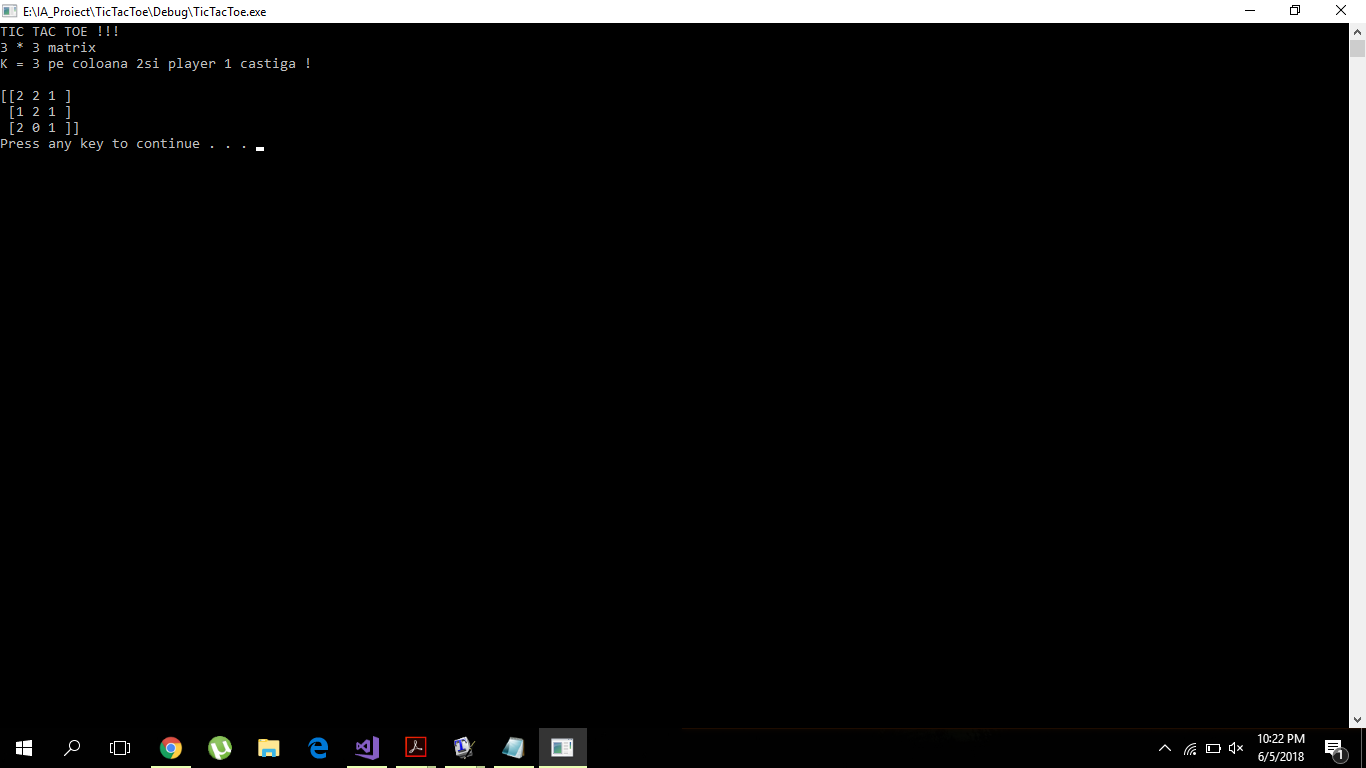
\includegraphics[scale=0.2]{prima.png}
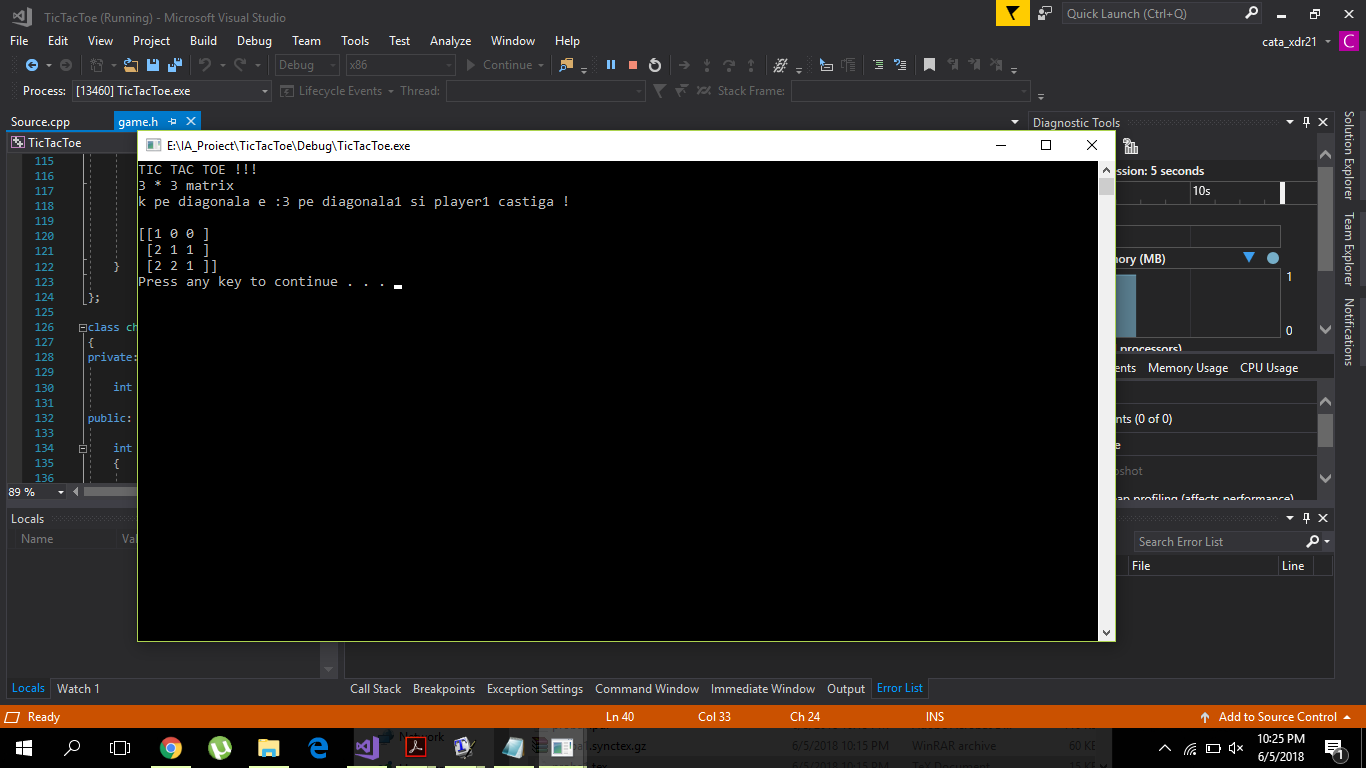
\includegraphics[scale=0.2]{adoua.png}
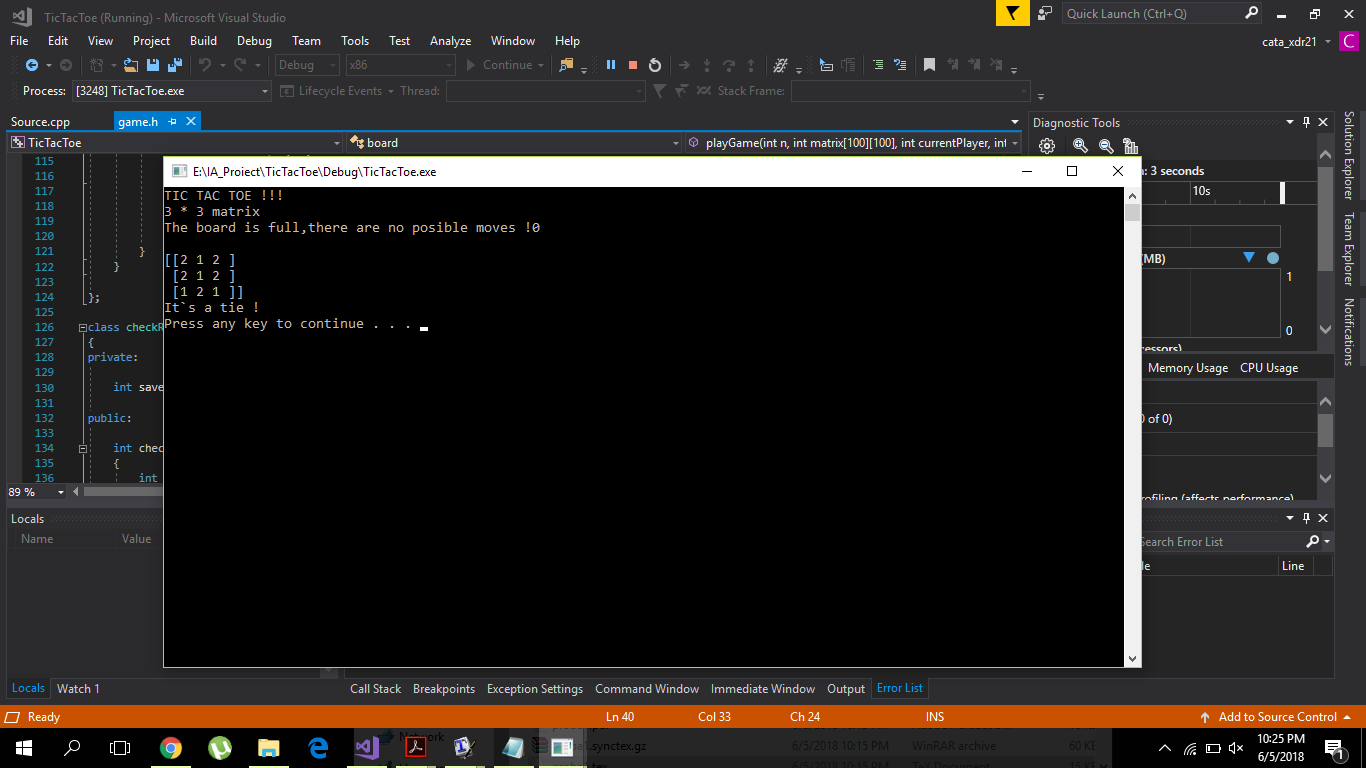
\includegraphics[scale=0.2]{atreia.png}










\end{document}
